% Preamble
\documentclass{article}
\usepackage{graphicx} % Required for inserting images
\usepackage{amsmath}

\title{PHYS506 $\LaTeX$}
\author{Eben Quenneville}
\date{September 17th 2024}


% Body
\begin{document}
\maketitle

\section*{Problem 0}
Hello World

\section*{Problem 1}
Euler's formula, given by $e^{ix} = \cos{x} + i \sin{x}$, establishes the fundamental relationship between the trigonometric functions and the complex exponential function.

\section*{Problem 2}
\begin{equation}\notag
	\int_{T_0}^{T_1} x^2 dx = \frac{1}{3} (T_{1}^{3} - T_{0}^{3})
\end{equation}

\section*{Problem 3}
\begin{equation}
	\delta x = \sqrt{\frac{1}{N(N-1)} \sum_{i=1}^{N} (x_i - \bar{x})^2}
\end{equation}

\section*{Problem 4}

\begin{center}
\begin{tabular}{|c|c|}
	\multicolumn{2}{c}{DMM Uncertainties} \\
	\hline
	DMM Model & MASTECH MS8268 \\
	\hline
	Resistance: & $\delta R = (1.2\%~~\text{of rdg + 2 digits})$ \\
	\hline
	DC Voltage: & $\delta V = (0.7\%~~\text{of rdg + 2 digits})$ \\
	\hline
	DC Current: & $\delta I = (1.2\%~~\text{of rdg + 3 digits})$ \\
	\hline
\end{tabular}
\end{center}

\newpage
\section*{Problem 5}

\begin{figure}[h]
    \centering
    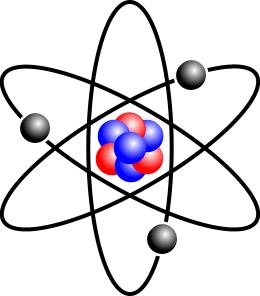
\includegraphics[width=0.3\textwidth]{atom.png}
    \caption{A picture of an atom.}
\end{figure}

\end{document}
